\documentclass[12pt]{article}
\usepackage{amsmath}
\usepackage{graphicx}
\usepackage{caption}
\usepackage{subcaption}

\begin{document}
\section{Data Analysis}
\subsection{Introduction}
We look for a signal due to the decay of axions to photons in the presence of a strong magnetic field. We assume that the axion has a close to Maxwellian distribution with energy fractional width of $\mathcal{O}(10^{-6}$, or about one 34 KHz bin. Raw FFT power spectra output from the measurement have their baselines subtracted, and are then combined to optimize sensitivity to a possible signal depositing excess power into a bin.

In section 4.2 we show the procedure for correcting the raw data and and cuts and fits that were applied. Section 4.3 discusses the power combining and resulting exclusion limit, section 4.4 describes the resulting candidates and section 5 shows our final exclusion result.

\section{Data Processing}
We will here describe the cuts applied to the raw data and fitting.

\subsection{Raw Data}

The measurements from Dec 2013 to May 2014 were taken at 368 distinct resonant frequencies, with 499 total observations made. 415 of these observations were taken for 1.06 hours, with a smaller number (28) being taken for longer observation times; the remaining observations were taken for shorter times. For each measurement we tracked the in-phase and quadrature components of the baseband signal, and converted the time-domain data into a 294 bin,  34013.6 Hz/bin double-sided FFT power spectra. The FFT traces are 10 MHz wide, with a center frequency at 0Hz. Each of the spectra are 500,000 averages lasting a total of 57 seconds in integration time; for the standard observation length of 1.06 hrs, there were 261 such spectra could be produced. 

\begin{figure}[h]
\centering
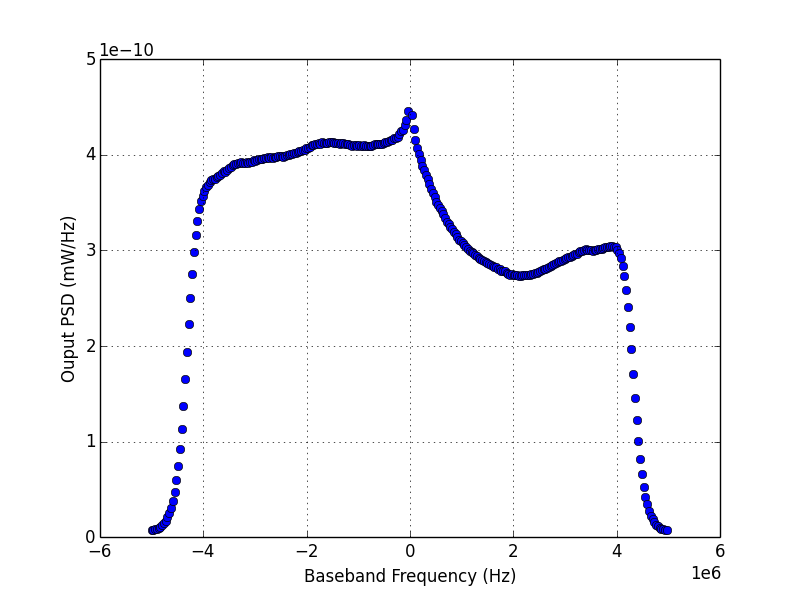
\includegraphics[width=\textwidth]{examplespectra}
\label{fig:example}
\caption{FFT Power spectral density vs baseband frequency. Each bin is 34013.6 Hz wide.}
\end{figure}

Shown in Figure\ref{fig:example} is one such raw FFT trace. The horizontal axis shows the baseband frequency, and the vertical axis corresponds to the power density across the 50 ohm input in milliWatts per Hz. The visible features in the spectrum are the spike at 0 Hz, which is DC noise, the skirts at the edges showing the attenuation of the last low pass filter in the receiver chain, the 1/f noise near the center, and a dip corresponding to the combined cavity-amplifier response.

\subsection{Corrections}

To remove the features due to the last low-pass filter, we cut out the first thirty and last thirty bins of each trace to remove the filter skirts, and also cut out twenty bins around the center to remove the DC spike and 1/f noise. 

At this point we do not correct for the total receiver transfer function. 

\begin{figure}[h]
\centering
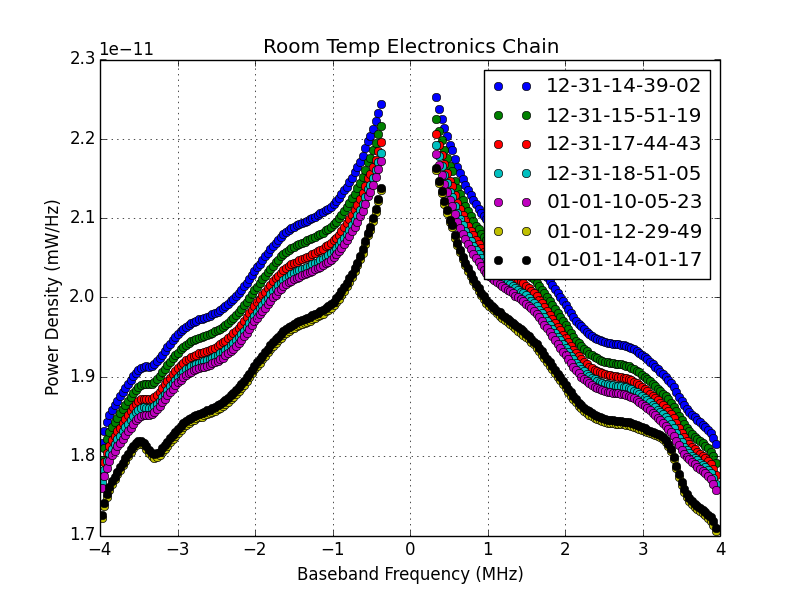
\includegraphics[width=\textwidth]{roomtempchain1}
\label{fig:roomtempchain1}
\caption{The transfer function of the room temperature electronics chain with the RF switch in place, for different settings of the first local oscillator.}
\end{figure}

Measurements of the room temperature electronics chain only (with the cryogenic amplifiers powered off) produce the FFT power spectra shown in Fig\ref{fig:roomtempchain1}. 

The variation in the amplitude of the room temperature receiver transfer function is approximately 20$\%$.

The first local oscillator of the receiver is usually set so that the cavity resonant frequency is mixed down to 2 MHz. However, there was a period of runs where the first local oscillator was set too high, so that the cavity frequency appeared at -1 MHz or -0.5 MHz in the baseband. There are also some measurements that had to be discarded because the local oscillator frequency was incorrectly set due to operator error and thus the cavity frequency was outside of the pass-band of the last filter. In order to prevent this from occurring, we introduced a test tone signal at an RF frequency such that it would mix down to -1 MHz, to make sure the local oscillator was set correctly. For the measurements taken with the test tone on, we later also cut out the bin with the test tone signal, as well as the two adjacent bins, for reasons to do with the fit.

\begin{figure}[h]
\begin{subfigure}{0.5\linewidth}
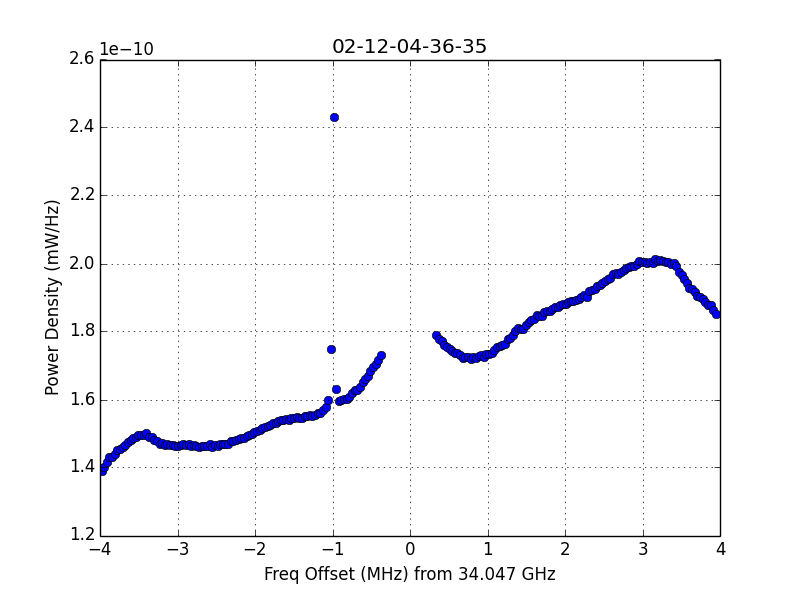
\includegraphics[width=\textwidth]{rawwithtesttone}
\caption{FFT trace with test tone signal at 34.044 GHz, -60 dBm}
\end{subfigure}
\begin{subfigure}{0.5\textwidth}
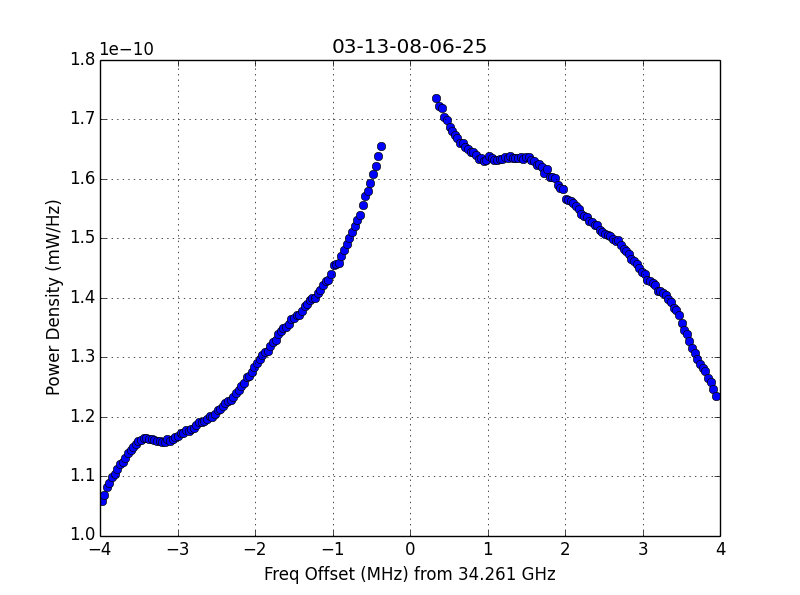
\includegraphics[width=\textwidth]{rawwithtesttone2}
\caption{FFT trace with test tone signal at 34.258 GHz, -72 dBm}
\end{subfigure}
\label{fig:testtone}
\end{figure}

\begin{figure}[h]
\centering
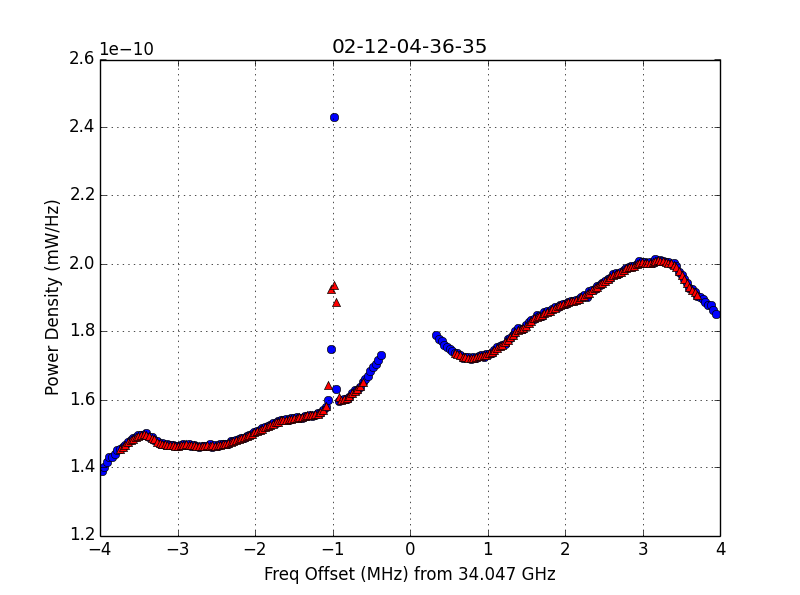
\includegraphics[width=0.85\textwidth]{rawwithfit2}
\label{fig:dataandfit}
\caption{FFT trace and fit.}
\end{figure}

We then fit the spectrum by computing the running average over every 3 bins, and cut the seven bins at the end of the spectrum as well as the seven bins nearest the gap. This is to guard against end effects when computing the running average. this smoothed curve is subtracted from the data to give our residual baseline.

\begin{figure}[h]
\centering
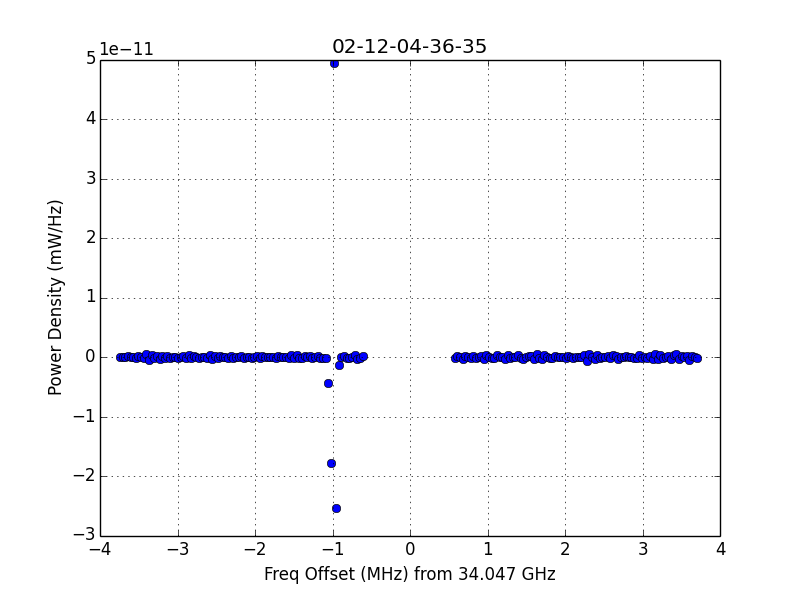
\includegraphics[width=0.85\textwidth]{meansub}
\label{fig:ms}
\caption{Residual}
\end{figure}

For the measurements taken with the cavity centered at 2 MHz, we discard the bins corresponding to negative frequencies in the FFT traces. Likewise, when the cavity resonance was mixed down to negative frequencies we neglect the bins corresponding to positive frequencies.

\begin{figure}[h]
\centering
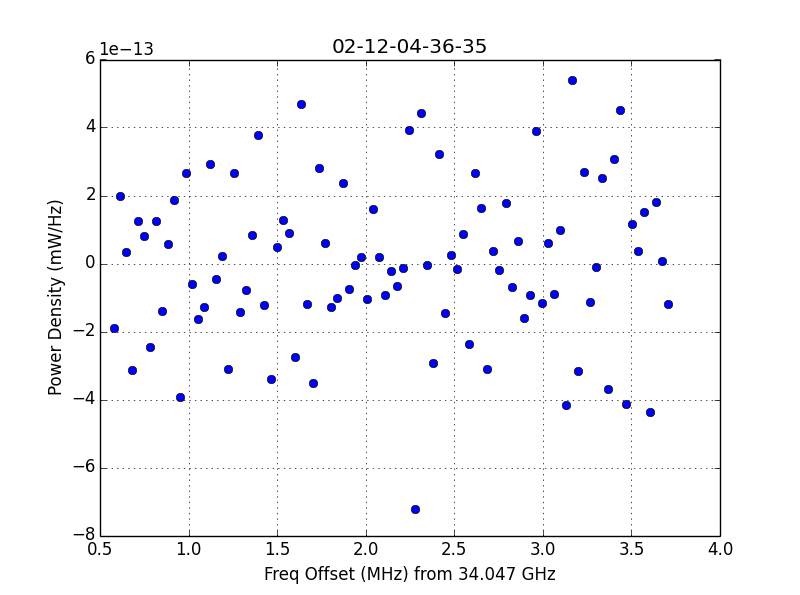
\includegraphics[width=0.85\textwidth]{meansubzoomed}
\label{fig:msz}
\caption{Residual zoomed in on cavity}
\end{figure}


The shape of the data near the cavity resonance is dictated by the interaction of the cavity and amplifier coupling.
\newpage

\begin{figure}[ht]
\begin{minipage}{0.5\linewidth}
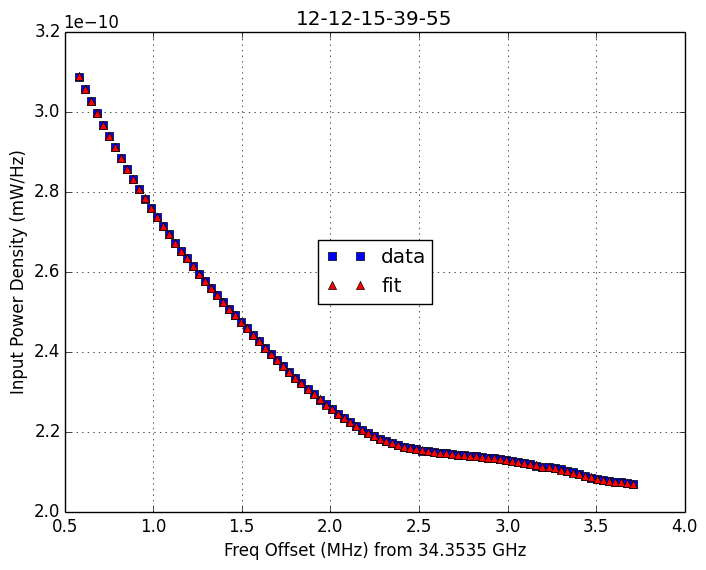
\includegraphics[scale=0.38]{12-12-15-39-55withfitposfreq_261}
\vspace{4ex}
\end{minipage}
\begin{minipage}{0.5\linewidth}
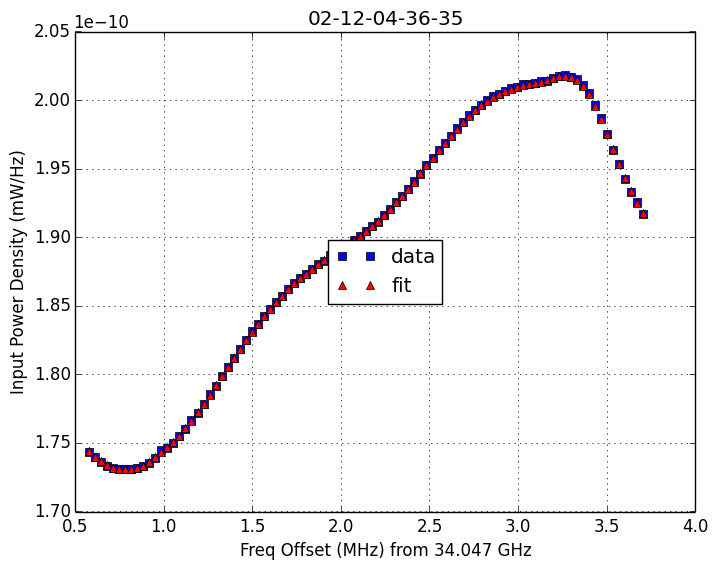
\includegraphics[scale=0.38]{02-12-04-36-35withfitposfreq_75}
\vspace{4ex}
\end{minipage}
\begin{minipage}{0.5\linewidth}
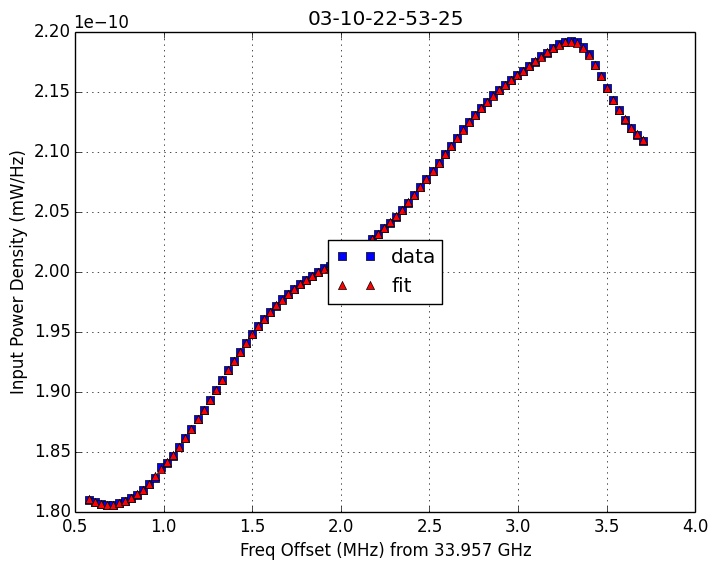
\includegraphics[scale=0.38]{03-10-22-53-25withfitposfreq_261}
\vspace{4ex}
\end{minipage}
\begin{minipage}{0.5\linewidth}
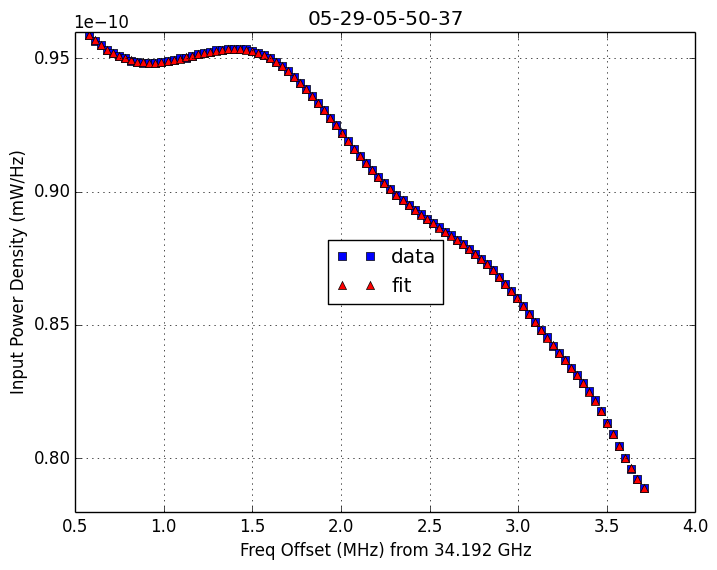
\includegraphics[scale=0.38]{05-29-05-50-37withfitposfreq_261}
\vspace{4ex}
\end{minipage}
\label{fig:varofcurve}
\caption{Data with fits for different resonant frequencies}
\end{figure}

 Refs REFYUTHESIS REFDAWTHESIS describe the equivalent circuit model of the cavity and amplifier. The result is a five parameter model that can be used to fit the measured data. We are able to fit the data successfully using the five parameter model, but find practically that the empirical fit is more convenient to use. 

PICOFFITWITH5PARAMMODEL

The $\delta P$ power fluctuations that result from the fit subtraction form the data that we analyze to look for excess power.

After subtracting the fit from each FFT trace, we average together many such corrected FFT traces. Within the standard observation time of 1.06 hrs, there were usually 261 FFT traces. Because temperature and pressure variations could cause the cavity frequency to shift during the hour of data taking as discussed in the previous chapter, all the FFT traces produced were inspected, and if there was a significant shift in the structure of the traces over the hour, those significantly different traces were discarded. 

\begin{figure}[h]
\centering
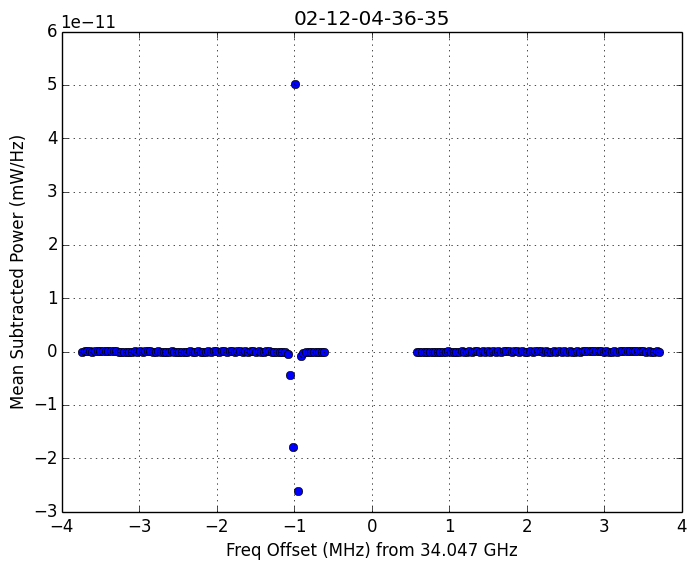
\includegraphics[width=0.85\textwidth]{02-12-04-36-35avgsubplt_75}
\label{fig:avgsubplt}
\caption{Average of 75 residual traces.}
\end{figure}

There is also leakage at the level of $0.5\%$ of the test tone power into the bins near 1 MHz. 

\begin{figure}[h]
\centering
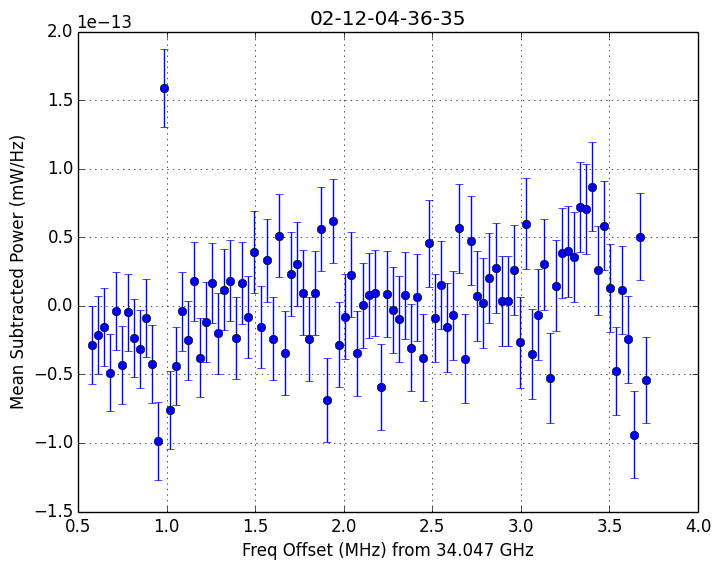
\includegraphics[width=0.85\textwidth]{02-12-04-36-35avgsubpltposfreq_75}
\label{fig:avgsubpltpos}
\caption{Average of 75 residual traces, zoom on region of interest.}
\end{figure}

This is due to incomplete isolation in the IQ mixer, which is responsible for separating out the in-phase and quadrature components of the signal. The test tone was present in 105 measurements. We gradually reduced the power level of the test tone, but for 72 of the observations, the leakage was visible and so we cut the the three bins around 1 MHz as well as the three bins around -1 MHz.

%\begin{figure}[h]
%\begin{subfigure}{0.5\linewidth}
%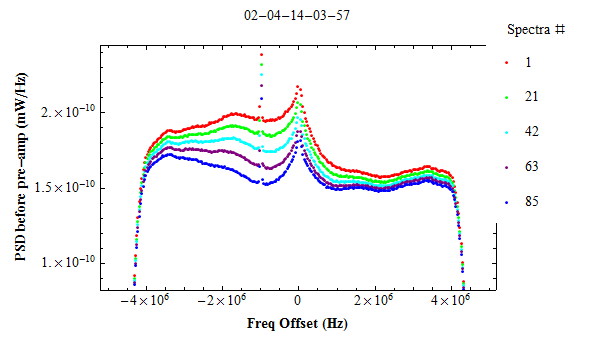
\includegraphics[width=1\textwidth]{02-04-14-03-57}
%\caption{Change in power spectra over course of 20 min run.}
%\end{subfigure}
%\begin{subfigure}{0.5\linewidth}
%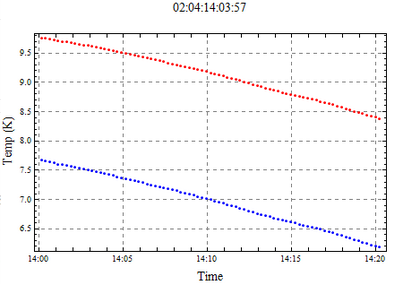
\includegraphics[width=0.8\textwidth]{temp02-04-14-03-57}
%\caption{Temperature of system (red = 1st amplifier, blue = cavity) over run.}
%\end{subfigure}
%\label{fig:tempdrift}
%\caption{We discard data when temperature drifts or frequency drifts occur.}
%\end{figure}

The distribution of fluctuations in the corrected and cut power spectra for one observation, averaging over all the FFT Traces, seems gaussian.

\begin{figure}[h]
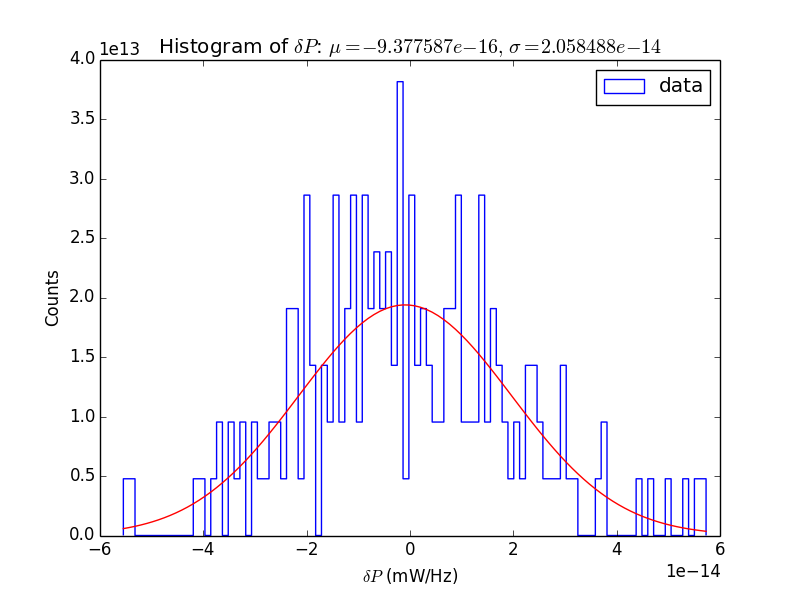
\includegraphics[width=\linewidth]{singlegaussian}
\label{fig:singlegaussian}
\caption{Histogram of the residual baseline after averaging 261 corrected FFT traces within the observation timestamp 12-18-21-01-03. The red is a gaussian fit to the histogram.}
\end{figure}

As we average the corrected FFT traces together, the fluctuations should go down as $t^{-1/2}$, or as the number of averages $1/\sqrt{N}$. To estimate this, we take the bins which do not survive the final cut of ``region of interest``; that is to say, for a cavity centered at 2 MHz, we take the residual baseline portion for the negative frequency bins, and by calculating the standard error of the mean as a function of the number of averaged FFT traces that go into the residual baseline, we can get an estimate of whether the system is behaving according to Gaussian statistics. The reason we take the negative (or opposite) frequency bins is to make sure we are only looking at background noise.

\begin{figure}[h]
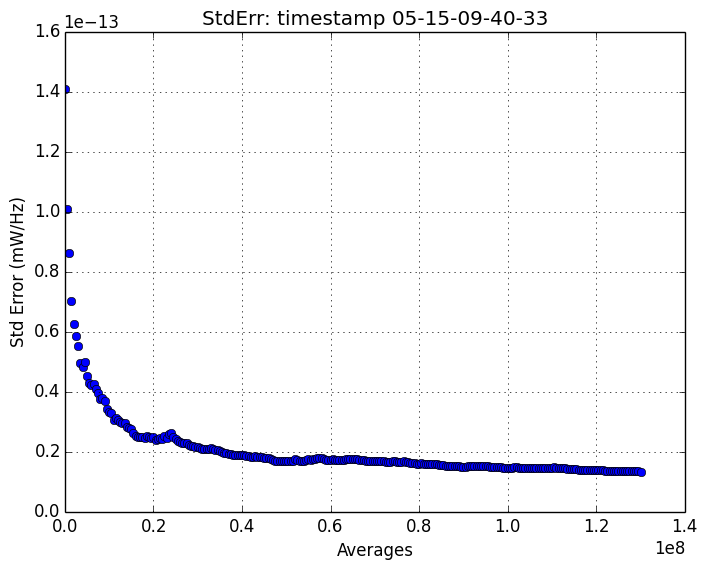
\includegraphics[width=\linewidth]{05-15-09-40-33stderrplt_261}
\label{fig:stderr}
\caption{The standard error of the mean of the background bins (92 bins) vs number of averages}
\end{figure}

The residual baseline for many runs shows a systematic error, showing that we have not fully removed all structure. The amplitude of this effect appears at the level of $0.1\%$.

\section{Combining Power Spectra}

For power spectra with overlapping frequency bins, we co-add the spectra at these bins by first dividing out the cavity shape, which is a lorentzian with peak at the cavity resonance frequency and bandwidth given by measurements prior to the observation. This ensures that the signal we expect to see will have nearly the same height in all bins (as all other variables affect the signal strength: form factor, Q, and frequency, are slowly varying compared to the lorentzian).




=====
BELOW THIS POINT IS OLD WORK

We used a cylindrical cavity cooled to $\sim 5$ K resonant at a frequency of $33.9-34.5$ GHz in the $\text{�}_{020}$ mode. The cavity was tuned to a specific resonant frequency using a dielectric rod; we measured the resonant frequency and Q using a vector network analyzer, then recorded the amplified noise from the cavity (after being mixed down to baseband) for an hour before retuning the cavity by 3 MHz. The baseband noise when Fourier transformed is a measure of the power in each frequency interval $\delta f$ that is the sum of the power in the cavity plus additional noise from the receiver chain. 

We recorded data in twelve separate runs (Nov 19 to May 30, 2014), and measured noise for 500 settings of the cavity frequency, with an hour of integration. The actual performance of our system

Summary of Runs
\begin{center}
\begin{tabular}{c | c | c }\hline
\hline
Run & No. of Freq.'s & State \\ \hline \hline
11/19-11/22 & 9 & slow DAQ \\ \hline
12/03-12/07 & 39 & faster DAQ \\ \hline
12/10-12/13 & 22 & tuning rod froze\\ \hline
12/16-12/20 & 27 & --\\ \hline
01/08-01/11 & 46 & heater feedback loop online\\ \hline
01/14-01/18 & 69 & RF switch added \\ \hline
01/23 & 5 & -- \\ \hline
01/28-02/01 & 41 & test tone added \\ \hline
02/04-02/07 & 33 & tuning rod froze\\ \hline
02/11-02/13 & 19 & -- \\ \hline
03/10-03/13 & 16 & -- \\ \hline
05/06-05/09 & x & weak coupling port altered, test tone removed\\ \hline
05/14-05/17 & x & -- \\ \hline
05/28-05/30 & x & -- \\ \hline
\hline
\end{tabular}
\label{table:runsummary}
\end{center}
\section{Procedure}
the following section is formed of quotes/notes from Silk(?) in "Inner Space Outer Space"
We tracked the in-phase and quadrature voltage of our baseband signal for an hour at each frequency setting. To allow for overlap between the covered frequencies, the cavity resonance was shifted by 3 MHz at a time. The dominant systematic effects were temperature variations in the cryostat. 

To reduce the effects of the the temperature shifts we discarded all data that was greater than 28 sigma away from the first minute of data. 

The data presented here were taken during 2014 Nov 19-22, Dec 05 to 07, 11 to 13, � . These runs gave a total of 500 hours of useful data. After correcting the data for the gain of the receiver and converting them to thermodynamic temperatures we compute the mean values $\Delta T_{bin}^i$ for the observations of each frequency bin of width $\delta f$ for each spectrum. The corresponding standard deviations, $\sigma_{bin}^i$ are calculated from the scatter of the individual 57 second measurements and are an estimate of the statistical uncertainty in the mean of an hour of data. ADDINBOOTSTRAP A typical value for data taken at 5 K is $\sigma_{bin189}^i = 0.25 mK$ whereas one expects $0.14$ mK from system noise alone. The excess noise at this stage is due to the $1/f$ component and in the variable temperature noise.

The final values $\bar \Delta T_{bin}^i$ for each one of the bins were obtained by weighting by $(\sigma_{bin}^i)^2$ each one of the hour observations for a given bin. The results are plotted in Figure 1 and show no statistically significant signal in any of the bins. The errors associated to each point correspond to the standard deviations estimated from the measurement statistics in the usual way. As the data will be used to decide what level of axion coupling is excluded by these measurements it is crucial to estimate the errors in Figure 1 accurately. The scatter in the values of $\Delta T_f^i$ for the different measurements could be larger than expected from the systematic effects. In principle, one could perform standard Chi-square tests for each one of the bins. Any such test would compare the scatter of the different observations of a given field with respect to the final value, with the corresponding values of $\sigma$. Let me emphasize that such a test does not depend on whether there is a true signal coming from the sky, as the scatter is computed with respect tone "local mean"; it is truly an instrumental Chi-square test. Figure 2 shows a histogram of the weighted residuals $(\Delta T - \bar \Delta T)\sigma$ for the observations. The histogram is reasonably gaussian with the a width that is consistent with what we would expect if all the scatter the values of $\Delta T$ with respect to their corresponding average value were due to fluctuations contained in $\sigma_i$. Indeed, the corresponding value of Chi-Square is of 78 with 75 degrees of freedom. Therefore, we conclude that it is legitimate to estimate the standard deviations $\bar \sigma$ in the standard way, as $\bar \sigma = [\Sigma \sigma^{-2}]^{-1/2}$. The variation of $\sigma$ frm bin to bin is mainly due to the different number of runs over which each frequency is observed. The weighted mean of the points in Figure 1 is $T_{avg} = 26 \pm 3 mk$.

It follows from visual examination of Figure 1 that none of the points differs significantly from the mean. The question is then what limits do the data place on $g_a$ from the fact that we only see the scatter shown in Figure 1. The Neyman-Pearson lemma prescribes the optimal statistical estimator for testing the hypothesis that $g_a \neq 0$. The optimal statistic turns out to be essentially a weighted Chi-square test, which can be used to find out which values of $g$ are ruled out at a certain confidence level.

\section{State Parameters}

Below is a plot of the measured loaded Q over the runs taken. NEED TO UPDATE
\begin{figure}
\centering
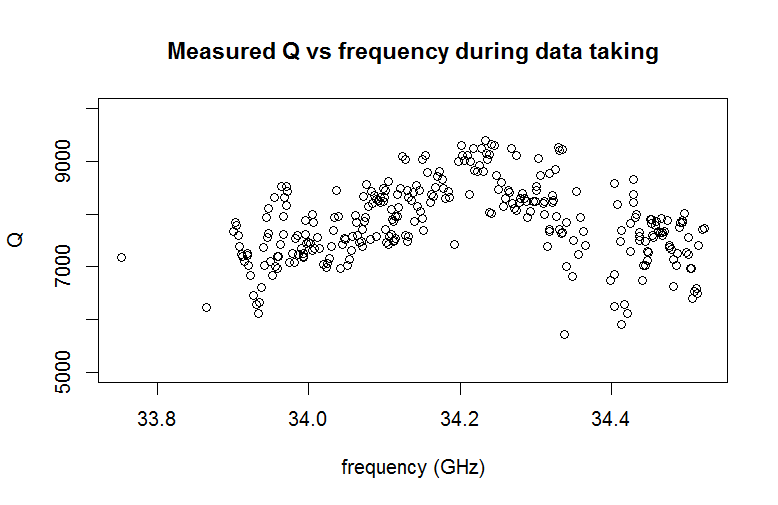
\includegraphics[width=1\textwidth]{measuredqvsfrequencyinsitucutoutoutlierswithtitle}
\end{figure}

Below is a plot of the form factor, calculated by simulating the electromagnetic fields in the cavity using the HFSS software.
\begin{figure}
\centering
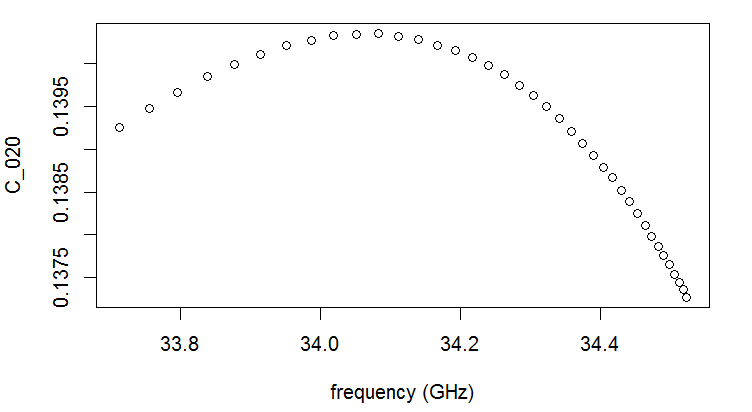
\includegraphics[width=1\textwidth]{formfactorvsfrequency}
\end{figure}

Shown below is a cross-sectional plot of the electric field in the z-direction for a dielectric rod with $\epsilon = 9.2$ inserted 0.028 inches into the cavity.

\begin{figure}
\centering
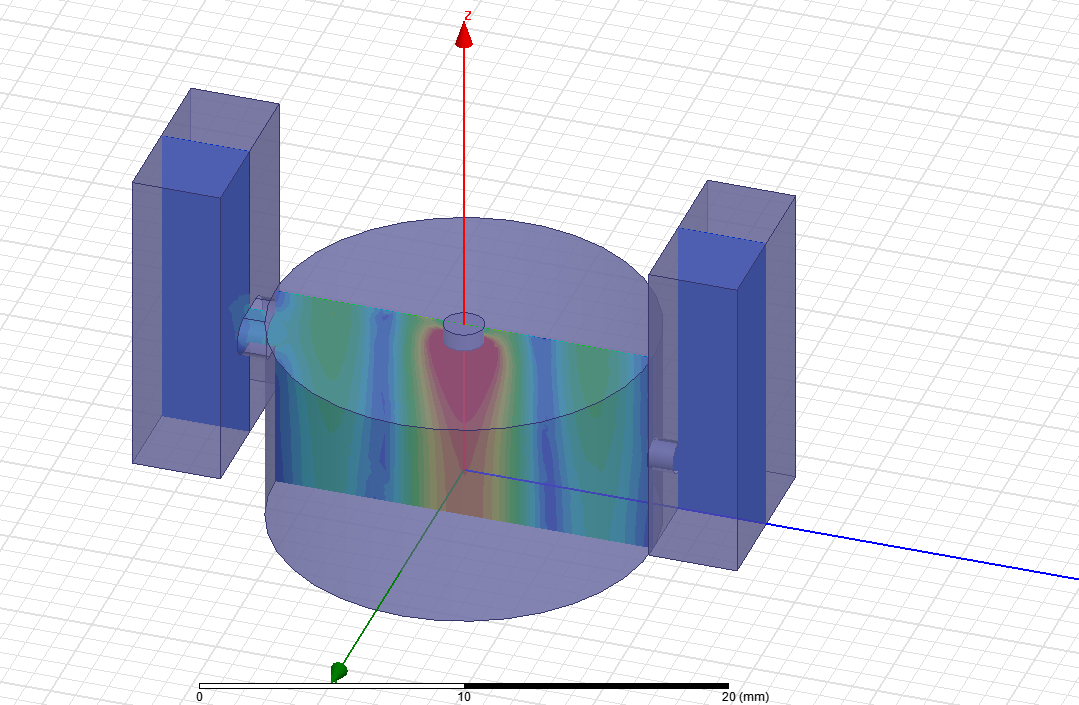
\includegraphics[width=0.8\textwidth]{efieldhfsssim28thou}
\end{figure}

Shown below is the frequency coverage NEED TO UPDATE

\begin{figure}
\centering
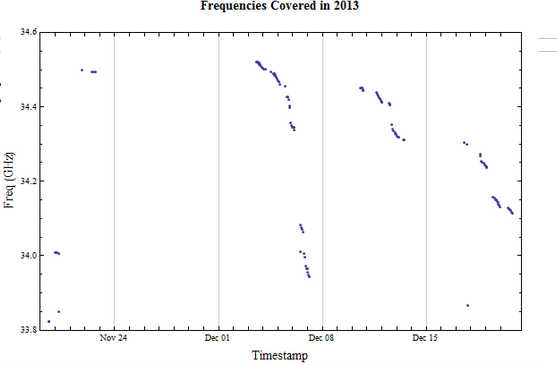
\includegraphics[scale=0.7]{frequencycoverage}
\end{figure}

\section{Data Analysis in Detail}
The data analysis starts from the raw time traces. The receiver chain at the final step separates the signal into an in-phase and quadrature component using an IQ mixer. These two separated signals each go through a low pass filter with approximately 4 MHz bandpass, and then are amplified by a voltage pre-amplifier with a gain of 5. The output channels (labeled henceforth as I and Q) are then plugged into a PCI 1154 card on a Dell desktop and digitized at a rate of 10 MSa/sec, with a a digital external referene at 10 MHz. We have a data acquisition program written in Visual C$\#$ that acquires however many records we desire, with each record containing 2.56e6 samples. The data acquisition has zero deadtime. The regular running procedure is to take 15,000 records at one particular cavity setting, and then retune - 15,000 records takes 1.06 hrs. 
Shown below is an example spectra

\begin{figure}
\centering
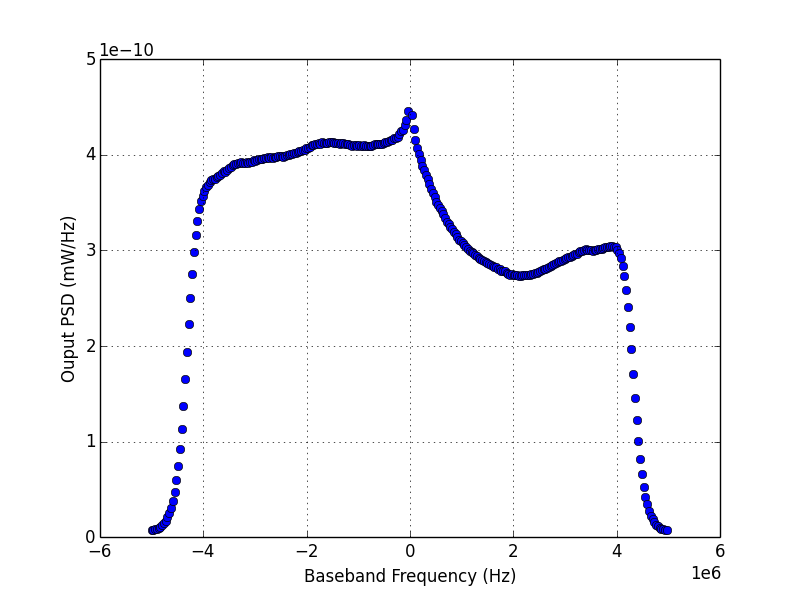
\includegraphics[width=\textwidth]{examplespectra}
\end{figure}

You can see the spike at 0 MHz which is our DC noise, the attenuation at the wings which is the result of the last 4 MHz Low-Pass filters, and the structure in the right hand side of the spectra, where the cavity is centered at 2 MHz. 

\subsection{cuts}

We discard all chunks that have the cavity drifting in frequency.

\begin{figure}
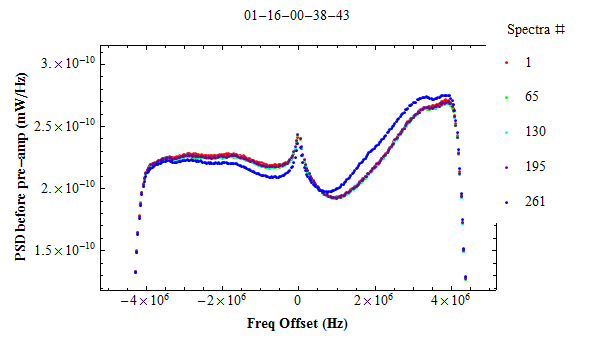
\includegraphics[width=\textwidth]{01-16-00-38-43}
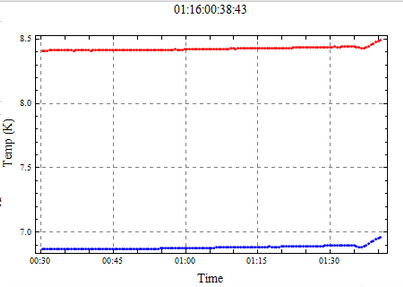
\includegraphics[width=\textwidth]{temp01-16-00-38-43}
\end{figure}
\begin{figure}
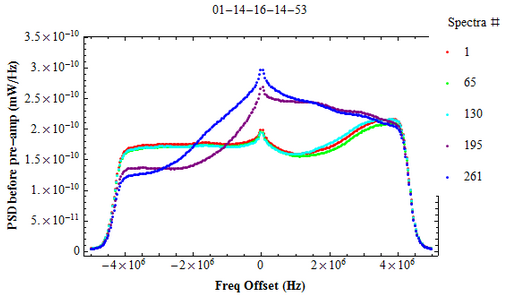
\includegraphics[width=\textwidth]{01-14-16-14-53}
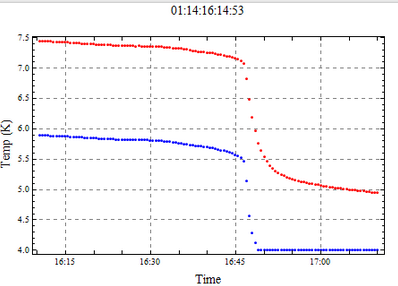
\includegraphics[width=\textwidth]{temp01-14-16-14-53}
\end{figure}

We also cut data when the temperature difference causes changes in the spectra.

\begin{figure}
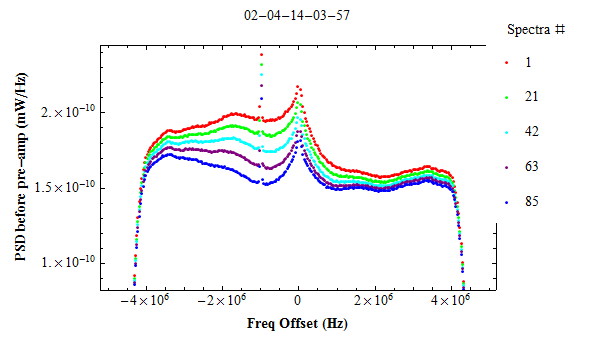
\includegraphics[width=\textwidth]{02-04-14-03-57}
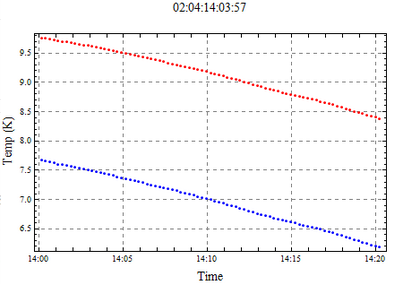
\includegraphics[width=\textwidth]{temp02-04-14-03-57}
\end{figure}
\begin{figure}
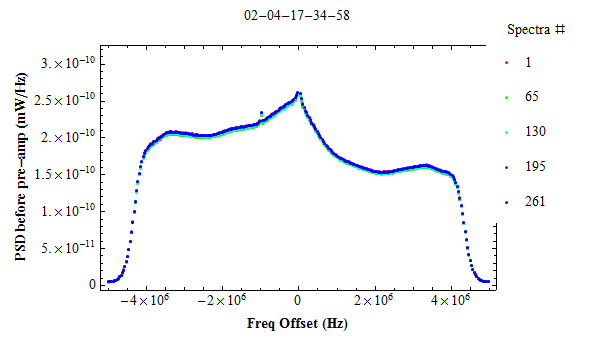
\includegraphics[width=\textwidth]{02-04-17-34-58}
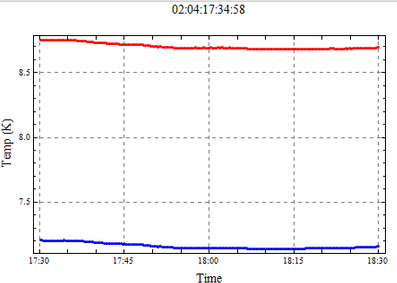
\includegraphics[width=\textwidth]{temp02-04-17-34-58}
\end{figure}

We take cuts on the data by removing the first 30 and last 30 points and also the 12 points in the middle where the DC spike occurs.

For runs taken after Jan 23, there was a test tone signal offset from the cavity resonance by -3 MHz to make sure we were seeing the correct structure. For these runs, the three bins centered on the test tone signal were cut as well. REALLY?

\centering 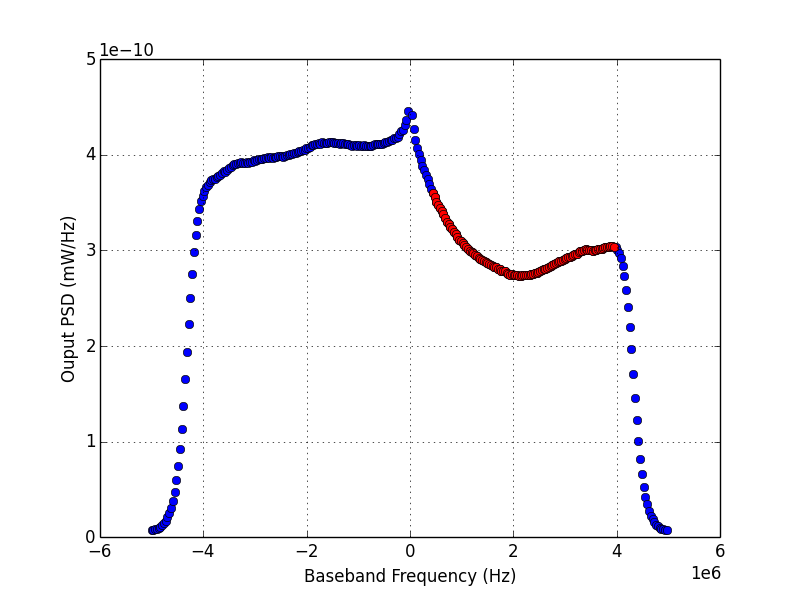
\includegraphics[width=0.6\textwidth]{cutondata}

We then do an empirical fit by smoothing the data using a moving average with window size of 3 bins. We subtract this smooth to get the fluctuations of the power spectrum about the local mean.

\begin{figure}
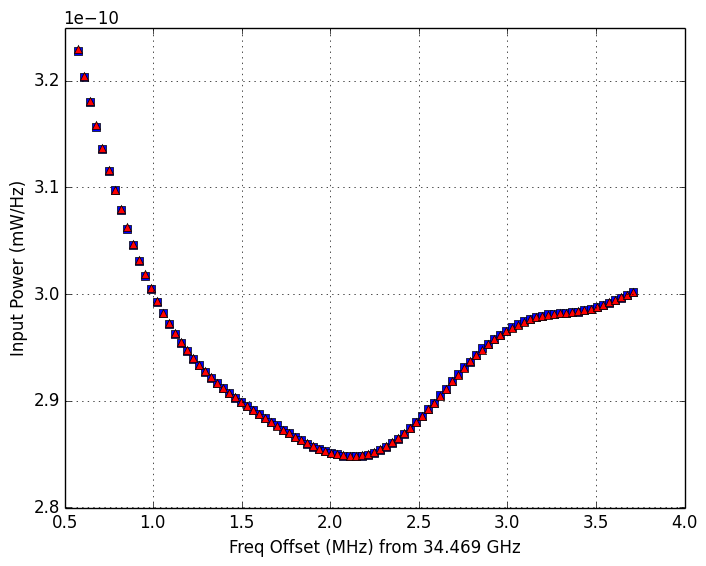
\includegraphics[width=0.8 \textwidth]{Dec04-11-33-24inputpltposfreq_237}
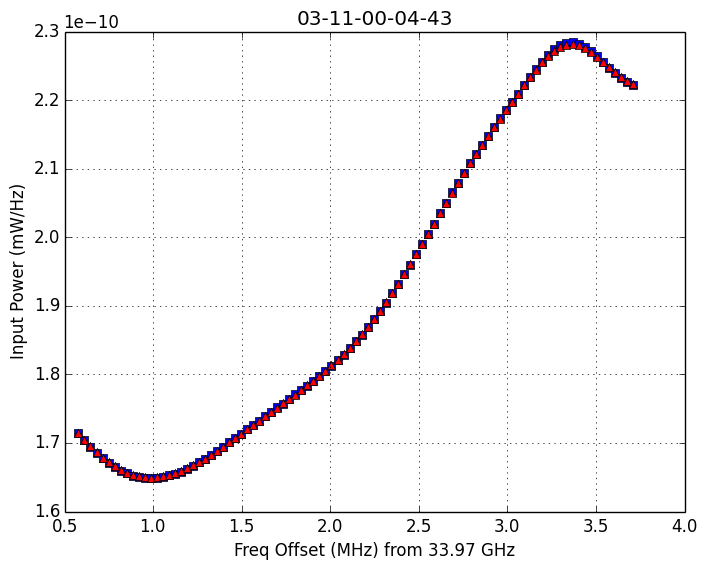
\includegraphics[width=0.8 \textwidth]{03-11-00-04-43inputpltposfreq_261}
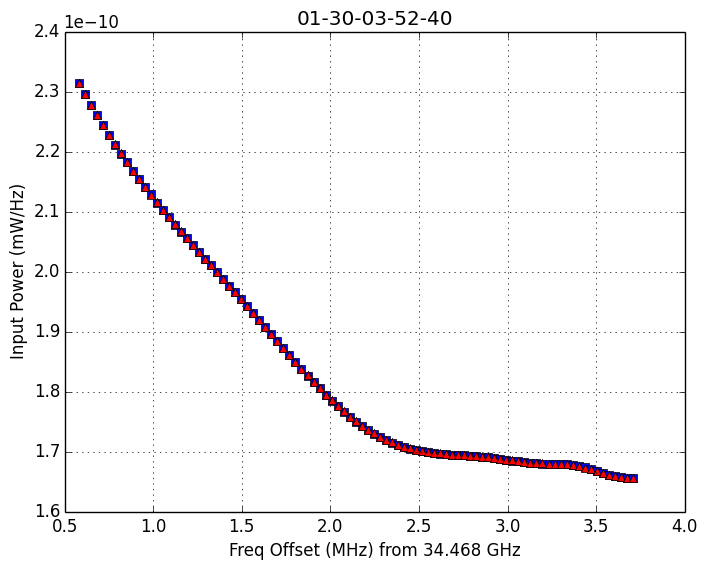
\includegraphics[width=0.8 \textwidth]{01-30-03-52-40inputpltposfreq_261}
\end{figure}

NEED TO UPDATE with figs with smooth (bin size  3). Here are the residuals of the subtraction for the above three timestamps: Point: shown here are the average of the residuals, where we discard spectra with significant temperature or frequency drifts. In the above timestamps, we were able to keep 90$\%$ of the data for the first timestamp, and all of the data for the second two.

\begin{figure}
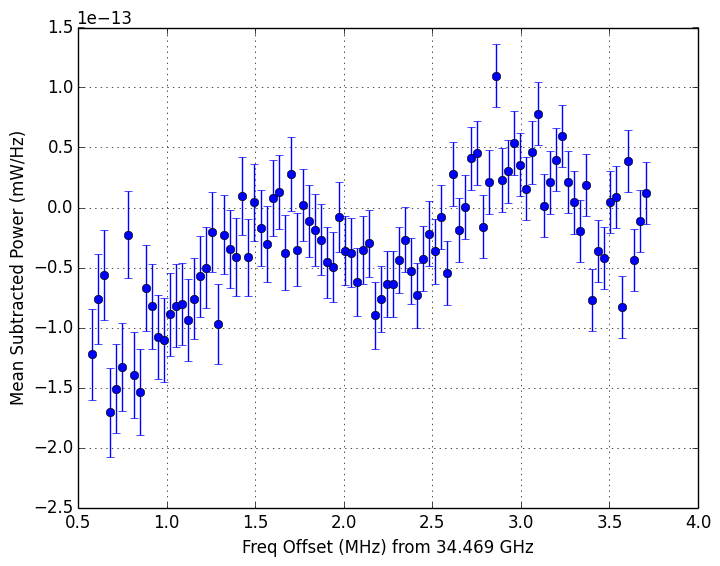
\includegraphics[width=0.8 \textwidth]{Dec04-11-33-24avgsubpltposfreq_237}
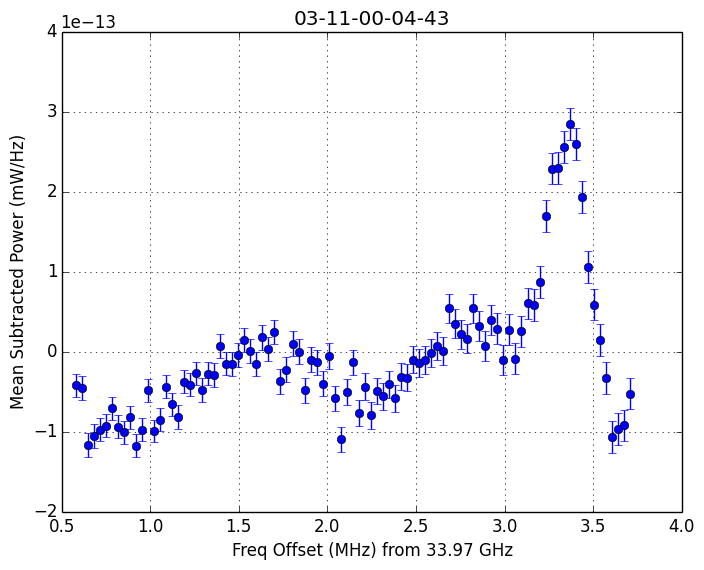
\includegraphics[width=0.8 \textwidth]{03-11-00-04-43avgsubpltposfreq_261}
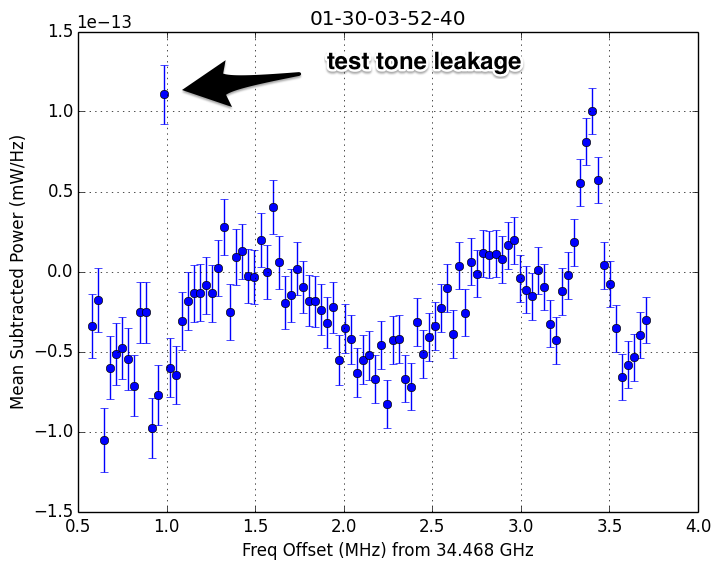
\includegraphics[width=0.8 \textwidth]{01-30-03-52-40avgsubpltposfreq_261}
\end{figure}

DIVIDE BY LORENTZIAN, COADD NEED TO UPDATE
Shown below is the excess power for an axion coupling of $g = 8.5 \times 10^{-11}$.

\begin{figure}
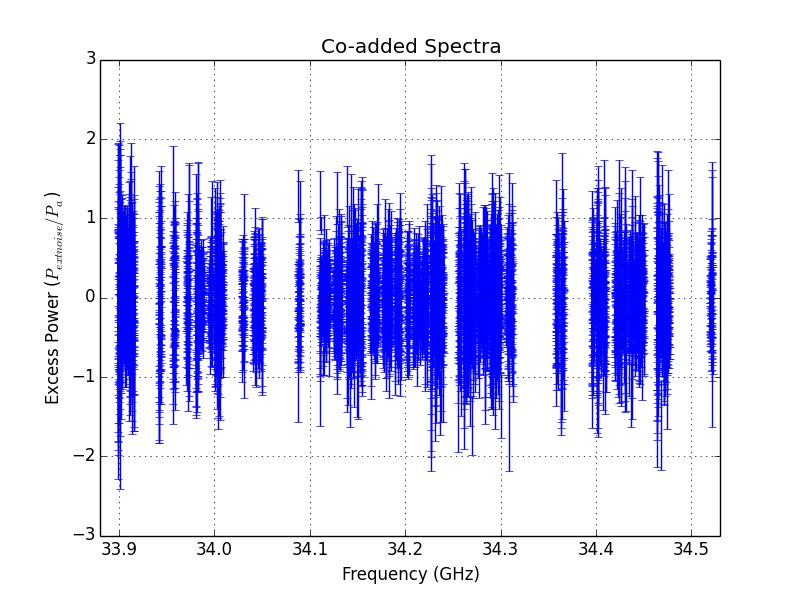
\includegraphics[width=\textwidth]{what}
\end{figure}

EXCLUSIONPLOT

\section{HFSS Design}

\includegraphics[width=\textwidth]{tableofchoice}

\includegraphics[width=0.6\textwidth]{tm020efield}

\includegraphics[width=0.6\textwidth]{tm020magneticfield}

\includegraphics[width=\textwidth]{waveguidefields}


\end{document}